
\section{Literature Review}

Process calculi (or process algebras) is a family of algebraic approaches to study concurrent systems \cite{historyPA}.  A process calculus need to address following questions:
\begin{inparaenum}[1.]
  \item What are primitive components in a concurrent system?
  \item What kind of computations and process behaviours could be modelled in this calculus?
  \item What does equivalence between two processes mean in this calculus?
\end{inparaenum}
In the past 30 years, a number of process calculi have been proposed and studied.  Each calculus answers the first two questions from slightly different perspectives.  For the third question, it is worth to note that a particular calculus may have more than one interpretation for process equivalences on different levels.

This chapter will present selective results in concurrent theories and their implementations.  \S\ref{sec:PA} will use the $\pi$-calculus as an example to sketch research topics in the area of process calculi, which provides formal basis for the design of concurrent languages.  \S\ref{sec:join} and \S\ref{sec:ambient} will focus on the programmability of the join-calculus and the ambient-calculus.  Both sections will introduce how to the subject calculus addresses problems in distributed programming and how ideas in the subject calculus are applied in real programming languages.  Algebraic properties of the subject calculus, however, will not be investigated in depth in this short review.  Then, \S\ref{sec:Erlang} will introduce OTP design principles which make distributed Erlang programs more reliable and maintainable.  \S\ref{sec:blue} will present indirect and direct encodings for the $\lambda$-calculus in process calculi.  Lastly, \S\ref{sec:vanroy} will give a short survey on a general framework for implementing concurrent programming languages.

\subsection{The $\pi$-calculus}
\label{sec:PA}

\subsubsection{Syntax and Notations}

The $\pi$-calculus \cite{pi_paper, pi_book} is a name passing calculus, in the sense that computations are represented by passing $\it{names}$ through $\it{channels}$.  The $\pi$-calculus uses lower-case letter to denote a name, which could be either a channel or a variable.  

Syntax of the $\pi$-calculus given in Table \ref{pi-syn} also denotes part of its semantics.  The prefix of a process denotes its capability, which could be  
\begin{inparaenum}[(i)]
  \item receiving names from a channel;
  \item sending names through a channel; or
  \item performing an internal action that cannot be observed from outside.
\end{inparaenum}
Informally, a process could :
\begin{inparaenum}[(1)]
  \item evolve to another process after performing an action;
  \item evolve as two processes who are running at the same time;
  \item evolve as one of the two processes;
  \item evolve to another process when two names become equal;
  \item a process with a private name;
  \item infinite parallel composition of the same process; or
  \item an inert process that does nothing.
\end{inparaenum}
Finally, two processes are structurally congruent, $\equiv$, if they are equal up to structure rules listed in Table \ref{pi-str-cong}

In the rest of this section, we distinguish reduction relation($\longrightarrow$) from labelled transition relations($\overset{\alpha}{\longrightarrow}$).  Specifically, the assertion $P \longrightarrow P'$ states that process $P$ can evolve to process $P'$ as a result of an action {\it{within}} $P$.  On the other hand, $P \overset{\alpha}{\longrightarrow} Q$ indicates that $P$ can evolve to Q after performing action $\alpha$.  Reduction relations are formally defined in Table \ref{pi-str-red} and transition relations are formally defined in Table \ref{pi-trans}.

\begin{table}[h]
  \begin{center}
  \begin{tabular}{ l c l  l l c l  l }
$\alpha$&:: = &                                                                    	& action           &P & :: =  & & process \\
              & $|$ & $u(\widetilde{x}$)                                       	& input            &   & $|$  & $ \alpha.P$&prefix\\
              & $|$ & $\overline{u} \langle \widetilde{y} \rangle$	& output          &   & $|$ &$P\ |\ P$& composition\\
              & $|$ & $\tau$                                                         	& silent/internal & & $|$ &$P\ +\ P$& summation\\
                                                                                                                 &&&&& $|$ &$ [x = y].P $& match \\
                                                                                                                 &&&&& $|$ & $(\mathit{\nu}x).P$&restriction\\
                                                                                                                 &&&&& $|$ & $!P$ & replication\\
                                                                                                                 &&&&& $|$ & 0 & inert process\\                                                                                                                 
  \end{tabular}
  \end{center}
  \caption{Syntax of the $\pi$-calculus}
  \label{pi-syn}
\end{table}

\begin{table}[h]
  \begin{center}
  \begin{tabular}{ l r c l }
  SC-MAT					&$[x = x] \alpha.P$			&$\equiv$&$\alpha.P$\\
  SC-SUM-ASSOC		&$P_1\ +\ (P_2\ +\ P_3)$	&$\equiv$&$(P_1\ +\ P_2)\ +\ P_3$\\
  SC-SUM-COMM		&$P_1\ +\ P_2$				&$\equiv$&$P_2\ +\ P_1$\\
  SC-SUM-INACT		&$P\ +\ 0$					&$\equiv$&$P$\\
  SC-COMP-ASSOC	&$P_1\ |\ (P_2\ |\ P_3)$	&$\equiv$&$(P_1\ |\ P_2)\ |\ P_3$\\
  SC-COMP-COMM		&$P_1\ |\ P_2$				&$\equiv$&$P_1\ |\ P_2$\\
  SC-COMP-INACT		&$P\ |\ 0$						&$\equiv$&$P$\\
  SC-RES					&$\nu z\ \nu w\ P$			&$\equiv$&$\nu w\ \nu z\ P$\\
  SC-RES-INACT		&$\nu z\ 0$					&$\equiv$&$0$\\
  SC-RES-COMP		&$\nu z\ (P_1\ |\ P_2)$		&$\equiv$&$P_1\ |\  \nu z\ P_2, if\ z\not{\in} fn(P_1)$\\
  SC-REP					&$!P$							&$\equiv$&$P\ |\ !P$\\
  \end{tabular}
  \end{center}
  \caption{The axioms of structural congruence}
  \label{pi-str-cong}
\end{table}

\vspace{20 mm}

\begin{table} [H]
  \begin{center}

  \begin{tabular}{ c c }
\multicolumn{2}{c}{R-INTER $\frac{}{(\bar{x}\langle y \rangle.P_1\ +\ M_1)\ |\ (x(z).P_2\ +\ M_2)\ \longrightarrow\ P_1\ |\ P_2\{y/z\}}$}\\
\\
R-PAR $\frac{P_1\ \longrightarrow\ P^{'}_{1}}{P_1\ |\ P_2\ \longrightarrow\ P^{'}_{1}\ |\ \ P_{2}}$ & 
R-RES $\frac {P\ \longrightarrow\ P^{'}} {\nu z P\ \longrightarrow\ \nu z P^{'}} $\\
\\
R-STRUCT $\frac {P_1\ \equiv\ P_2\ \ P_2\ \longrightarrow\ P_2^{'}\ \ P_2^{'}\ \equiv\ P_1^{'}\ } {P_1\ \longrightarrow\ P^{'}_{1}} $&
R-TAU $\frac {} {\tau  P\ + \ M\ \longrightarrow\ P}$
  \end{tabular}
  \end{center}
  \caption{Reduction rules in the $\pi$-calculus}
  \label{pi-str-red}
\end{table}

\vspace{10 mm}

\begin{table}[H]
  \begin{center}
  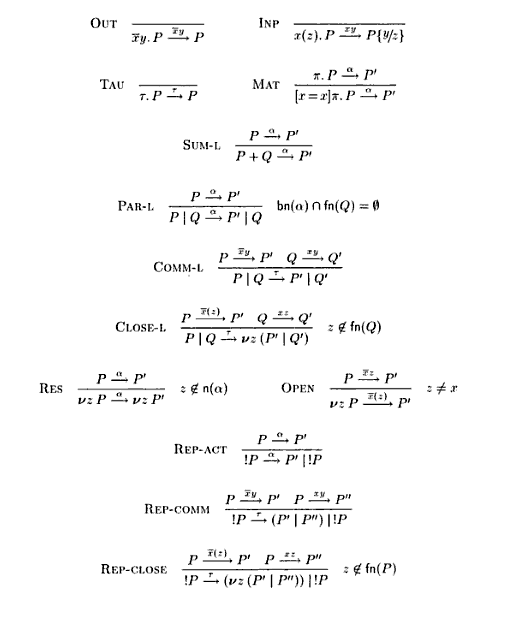
\includegraphics[scale=0.4]{pi_trans.png}
  \end{center}
  \caption{Transition rules in the $\pi$-calculus}
  \label{pi-trans}
\end{table}


\subsubsection{Equivalence Relations}

Equivalence relations are important concepts in an algebraic system.  Unfortunately, the variety of equivalence relations in the $\pi$-calculus and other classical process calculi are usually obstacles to learning a calculus.  This section will give a gentle introduction to the most important equivalence relation in the $\pi$-calculus, the strong barbed bisimulation, followed by short definitions cited from \cite{pi_book} in a designed order.  By reading this section, readers will obtain a basic understanding for all equivalences in the Figure \ref{pi-eq} and most other common equivalences in literature.


$\bf{Barbed\ relations}$ study the behaviour of a process via examining its potential interactions with the environment.  Formally,

\begin{defn}
For each name or co-name $\mu$, the observability predicate $\downarrow_\mu$ is defined by:\\
    (1) P $\downarrow_\mu$ if P can perform an input action via channel $\mu$\\
    (2) P $\downarrow_\text{$\overline{\mu}$}$ if P can perform an output action via channel $\mu$
\end{defn}
 
Strong barbed relations can be defined as follows:

\begin{defn}
A relation S is a $\mathbf{strong\ barbed\ bisimulation}$ if whenever (P,Q) $\in$ S,\\
(1) P $\downarrow_\mu$ implies Q$\downarrow_\mu$\\
(2) P $\overset{\tau}{\longrightarrow}$ P' implies Q $\overset{\tau}{\longrightarrow}$ Q' for some Q' with (P', Q') $\in$ S \\
(3) Q $\downarrow_\mu$ implies P$\downarrow_\mu$\\
(4) Q $\overset{\tau}{\longrightarrow}$ Q' implies P $\overset{\tau}{\longrightarrow}$ P' for some P' with (P', Q') $\in$ S
\end{defn}

\begin{defn}
P and Q are $\mathbf{strong\ barbed\ bisimilar}$ if (P,Q) $\in$ S for some barbed bisimulation S.
\end{defn}

\begin{defn}
P and Q are $\mathbf{strong\ barbed\ congruence}$ if C[P] and C[Q] are strong barbed bisimilar for any context C\footnote{A context, $C[\cdot]$ is a term written using the same syntax of the $\pi$-calculus and an additional constant $\cdot$.  Substituting the $\cdot$ by a process P result in a $\pi$-calculus term $C[P]$ }.
\end{defn}

\begin{defn}
P and Q are $\mathbf{strong\ barbed\ equivalent}$ if P $|$ R and Q $|$ R are strong barbed bisimilar for any process R.
\end{defn}

$\bf{Bisimulation,\ bisimilarity,\ congruence,\ and\ equivalent}$, as revealed in the barbed relations, are four related concepts in process calculi.  For this reason, in the rest of this subsection, where various of equivalent relations will be introduced, only one of the four concepts in each group will be defined explicitly.  The meaning of the rest three relations in each group should be apparent. 

\begin{defn}
A relation S is a $\mathbf{reduction\ bisimulation}$ if whenever (P,Q) $\in$ S,\\
(1) P $\overset{\tau}{\longrightarrow}$ P' implies Q $\overset{\tau}{\longrightarrow}$ Q' for some Q' with (P', Q') $\in$ S \\
(2) Q $\overset{\tau}{\longrightarrow}$ Q' implies P $\overset{\tau}{\longrightarrow}$ P' for some P' with (P', Q') $\in$ S
\end{defn}

In terms of evaluation strategy, the $\pi$-calculus could adopt either the early instantiation scheme or the late instantiation scheme.  In the early instantiation scheme, variables are instantiated as soon as an input message is received, more precisely, $\frac{-}{a(x).P\ \overset{av}{\longrightarrow}P\{v/x\}}$.  On the contrary, in the late instantiation scheme, bound variables of input actions are instantiated only when they are involved in an internal communication.

\begin{defn}
A binary relation S on processes $P$ and $Q$ is an $\mathbf{early\ simulation}$, $\sim_e$,  if PSQ implies that\\
1. If P $\overset{\alpha}{\longrightarrow}$ P' and $\alpha$ is a free action\footnote{an internal action or a free output.}, then for some Q', Q $\overset{\alpha}{\longrightarrow}$ Q' and P'SQ'\\
2. If P $\overset{x(y)}{\longrightarrow}$ P' and y$\not{\in}$ n(P,Q), then for all w, there is Q' such that Q$\overset{x(y)}{\longrightarrow}$ Q' and P\{w/y\}SQ\{w/y\}\\
3. If P $\overset{\bar{x}(y)}{\longrightarrow}$ P' and y$\not{\in}$ n(P,Q), then for some Q', Q $\overset{\bar{x}(y)}{\longrightarrow}$ Q' and P'SQ'
\end{defn}

\begin{defn}
A binary relation S on agents is a $\mathbf{late \ simulation}$, $\sim_l$,  if PSQ implies that\\
1. If P $\overset{\alpha}{\longrightarrow}$ P' and $\alpha$ is a free action, then for some Q', Q $\overset{\alpha}{\longrightarrow}$ Q' and P'SQ'\\
2. If P $\overset{x(y)}{\longrightarrow}$ P' and y$\not{\in}$ n(P,Q), then for some Q', Q$\overset{x(y)}{\longrightarrow}$ Q' and for all w, P\{w/y\}SQ\{w/y\}\\
3. If P $\overset{\bar{x}(y)}{\longrightarrow}$ P' and y$\not{\in}$ n(P,Q), then for some Q', Q $\overset{\bar{x}(y)}{\longrightarrow}$ Q' and P'SQ'
\end{defn}

\begin{defn}
P and Q are $\mathbf{full\ bisimilar}$, P $\approx^c$ Q	, if P$\sigma\ \approx$ Q$\sigma$ for every substitution $\sigma$.
\end{defn}

\begin{defn}
A binary relation R over processes is an $\mathbf{open\ bisimulation}$, $\approx_o$, if for every pair of elements (p,q) $\in$ R and for every name substitution $\sigma$ and every action $\alpha$, whenever p$\sigma \overset{\alpha}{\longrightarrow}$ p' then there exists some q' such that q$\sigma\overset{\alpha}{\longrightarrow}$q' and (p', q') $\in$ R.
\end{defn}

\begin{defn}
A relation is $\mathbf{ground\ bisimulation}$, $\approx_g$, iff whenever P $\approx_g$ Q, there is z$\not{\in}$fn(P, Q) such that if P$\overset{\alpha}{\longrightarrow}$Q, where $\alpha$ is an action, then then Q$\overset{\alpha}{\Rightarrow }\approx_g$P.
\end{defn}

To conclude this subsection, Figure \ref{pi-eq}, cited from \cite{pi_book}, presents the hierarchy of equivalences in the $\pi$-calculus.

\begin{figure} [h]
  \begin{center}

\begin{picture}(100, 160)
  \put(90, 160){$weakest$}
  \put(100, 80){\vector(0,1){70}}
  \put(100, 80){\vector(0,-1){70}}
  \put(90, 0){$strongest$}
  
  \put(50,160){$\approx_g$}
  \put(60,130){\line(0,1){20}}
  \put(50,120){$\approx,\ \cong$}
  \put(45,90){\line(2,3){14}}
  \put(60,90){\line(0,1){20}}
  \put(0,80){$\approx_g^c,\ \approx^c,\ \cong^c$}
  \put(60,80){$\approx_l$}
  \put(45,55){\line(2,3){14}}
  \put(45,55){\line(0,1){20}}
  \put(45,40){$\approx_l^c$}
  \put(45,15){\line(0,1){20}}
  \put(45,0){$\approx_o$}
\end{picture}
  \end{center}

  \begin{center}
  \begin{tabular}{ c l c l c l}
$\approx_g:$&$ground\ bisimilarity$&$\approx:$&$bisimilarity$&$\cong:$&$barbed\ equivalence$\\
$\approx_g^c:$&$ground\ congruence$&$\approx^c:$&$full\ bisimilarity$&$\cong^c:$&$barbed\ congruence$\\
$\approx_l:$&$late\ bisimilarity$&$\approx_l^c:$&$late\ congruence$&$\approx_o:$&$open\ bisimilarity$\\
  \end{tabular}
  \end{center}
  \caption{Hierarchy of equivalences in the $\pi$-calculus}
  \label{pi-eq}
\end{figure}


\subsection{The Join-Calculus and the JoCaml Programming Language}
\label{sec:join}
%Join-calculus and JoCaml 12 - 14

Join-calculus \citep{RCHAM} is a name passing process calculus that is designed for the distributed programming.  There are two versions of the join-calculus, namely the core join-calculus and the distributed join-calculus.  The core join-calculus could be considered as a variant of the ${\pi}$-calculus.  It is as expressive as the asynchronous ${\pi}$-calculus in the sense that translations between those two calculi are well formulated.  A remarkable construct in the join-calculus is join patterns, which provides a convenient way to express process synchronisations.  This feature also makes the join-calculus closer to a real programming language.  The distributed join-calculus extends the core calculus with location, process migration, and failure recovery.  This proposal uses the short phrase ``join-calculus'' to refer to the distributed join-calculus which includes all components in the core join-calculus.  The syntax (Table \ref{join_syn}), the scoping rules (Table \ref{join_scope}), and the reduction rules (Table \ref{join_rule}) of the join-calculus are cited from \citep{join}.

\begin{table}[H]
  \begin{center}
  \begin{tabular}{ l c l  l l c l  l }
$P$  & :: =  &                                               & processes                      &$D$& :: =  & & definition \\
 & $|$ & $x \langle \widetilde{v} \rangle $   & asynchronous                 &&$|$&$J\ \triangleright \ P$&local rule\\
 & $ $ & $                                               $   & message                        &&$|$&$\top$             & inert definition\\
 & $|$ & $ \mathbf{def}\ D\ \mathbf{in}\ P$ & local definition                &&$|$&$D\ \wedge \ D$&co-definition\\
 & $|$ & $P\ |\ P$                                        & parallel                           &&$|$&$a\ [D\ :\ P]$& \bf{sub-location} \\
 & $ $ & $                                               $   & composition                   &&$|$&$\Omega a\ [D\ :\ P] $& \bf{dead sub-location} \\ 
 & $|$ & $\mathbf{0}$                                 & inert process                  &$J$& ::= & &join-pattern\\
 & $|$ & $go\langle a, \kappa \rangle$       & \bf{migration}                  &&$|$& $x\langle\widetilde{v}\rangle$ & message pattern\\
 & $|$ & $halt \langle \rangle $                   & \bf{termination}               &&$|$&$J|J$& synchronous \\
 & $|$ & $fail\langle a, \kappa \rangle $     & \bf{failure detection}        &&$$&$$&join-pattern\\

   \multicolumn{8}{p{\textwidth}}{Constructs whose explanation is in {\bf{bold}} font are only used in the distributed join-calculus.  Other constructs are used in both distributed and local join-calculus.}\\
  \end{tabular}
  \end{center}
  \caption{Syntax of the distributed join-calculus -- \citep{RCHAM} }
  \label{join_syn}
\end{table}

\begin{table}[h]
  \begin{center}
  \begin{tabular}{ r l c l  l  c l  }
  $J:$&$dv[x\langle\widetilde{v}\rangle]$&$\overset{def}{=}$&$\{x\}$& $rv[x\langle\widetilde{v}\rangle]$&$\overset{def}{=}$&$\{u \in \widetilde{v}\}$\\
  &$dv[J\ |\ J']$&$\overset{def}{=}$&$dv[J]\cup dv[J']$&$rv[J\ |\ J']$&$\overset{def}{=}$&$rv[J]\uplus rv[J']$\\
  $D:$&$dv[J\ \triangleright \ P]$&$\overset{def}{=}$&$dv[J]$&$rv[J\ \triangleright \ P]$&$\overset{def}{=}$&$dv[J]\cup(fv[P]-rv[J])$\\
  &$dv[\top]$&$\overset{def}{=}$&$\emptyset$&$fv[\top]$&$\overset{def}{=}$&$\emptyset$\\
  &$dv[D\ \wedge \ D']$&$\overset{def}{=}$&$dv[D]\cup dv[D']$&$fv[D\ \wedge \ D']$&$\overset{def}{=}$&$fv[D]\cup fv[D']$\\
  &$dv[a\ [D\ : P]]$&$\overset{def}{=}$&$\{a\} \uplus dv[D]$&$fv[a\ [D\ : P]]$&$\overset{def}{=}$&$\{a\} \cup fv[D] \cup fv[P]$\\
  $P:$&$fv[x\langle\widetilde{v}]$&$\overset{def}{=}$&$\{x\}\cup\{u\in\widetilde{v}\}$&$fv[go\langle a, \kappa \rangle]$&$\overset{def}{=}$&$\{a,\kappa\}$\\
  &$fv[\mathbf{0}]$&$\overset{def}{=}$&$\emptyset$&$fv[halt\langle\rangle]$&$\overset{def}{=}$&$\emptyset$\\
  &$fv[P\ |\ P']$&$\overset{def}{=}$&$fv[P]\cup fv[P']$&$fv[fail\langle a, \kappa \rangle]$&$\overset{def}{=}$&$\{a,\kappa\}$\\
  &$fv[ \mathbf{def}\ D\ \mathbf{in}\ P]$&$\overset{def}{=}$&\multicolumn{2}{l}{$(fv[P]\cup fv[D])-dv[D]$}\\
  \multicolumn{7}{p{\textwidth}}{Well-formed conditions for $D$: A location name can be defined only once; a channel name can only appear in the join-patterns at one location.}
  \end{tabular}
  \end{center}
  \caption{Scopes of the distributed join-calculus -- \citep{RCHAM} }
  \label{join_scope}
\end{table}

\begin{table}[h]
  \begin{center}
  \begin{tabular}{l r c l r}
  \bf{str-join}   &$\vdash\ P_1\ |\ P_2$&$\rightleftharpoons$&$\vdash \ P_1 ,\ P_2$\\
  \bf{str-null}   &$\vdash\ \mathbf{0}$&$\rightleftharpoons$&$\vdash$\\
  \bf{str-and}   &$D_1\ \wedge D_2\ \vdash$&$\rightleftharpoons$&$D_1,\ D_2\ \vdash$\\
  \bf{str-nodef}&$\top$&$\rightleftharpoons$&$\vdash$\\
  \bf{str-def}    &$\vdash\ \mathbf{def}\ D\ \mathbf{in}\ P$&$\rightleftharpoons$&$D\sigma_{dv}\ \vdash\ P\sigma_{dv}$&(range($\sigma_{dv}$) fresh)\\
  \bf{str-loc}    &$\varepsilon a\ [D\ :\ P] \vdash_\varphi$&$\rightleftharpoons$&$\vdash_\varphi\ \parallel\ \{D\}\ \vdash_{\varphi\varepsilon a}\ \{P\}$&($a$ frozen)\\
  \\
  \bf{red}&$J\ \triangleright \ P\ \vdash_\varphi\ J\sigma_{rv}$&$\longrightarrow$&$J\ \triangleright \ P\ \vdash_\varphi\ P\sigma_{rv}$&($\varphi$ alive)\\
  \bf{comm}&$\vdash_\varphi\ x\langle\widetilde{v}\rangle \  \parallel\ J\ \triangleright P \vdash\ $&$\longrightarrow$&$\vdash_\varphi\ \parallel\ J\ \triangleright P\ \vdash\  x\langle\widetilde{v}\rangle $&($x\in dv[J],\ \varphi$ alive)\\
  \bf{move}&$a[D\ :\ P|go\langle b,\kappa\rangle]\ \vdash_\varphi\ \parallel\ \vdash_{\psi\varepsilon b}$&$\longrightarrow$&$\ \vdash_\varphi\ \parallel\ a\ [D:P|\kappa\langle\rangle]\ \vdash_{\psi\varepsilon b}$&($\varphi$ alive)\\
  \bf{halt}&$a[D\ :\ P|halt\langle\rangle]\ \vdash_\varphi\ $&$\longrightarrow$&$\Omega a[D\ :\ P]\ \vdash_\varphi\ $&($\varphi$ alive)\\
  \bf{detect}&$\vdash_\varphi fail\langle a,\kappa\rangle\ \parallel\ \vdash_{\psi\varepsilon a}$&$\longrightarrow$&$\ \vdash_\varphi\ \kappa\langle\rangle\ \parallel\ \vdash_{\psi\varepsilon a}$&($\psi\varepsilon a$ dead, $\varphi$ alive)\\
    \multicolumn{5}{p{\textwidth}}{Side conditions: in {\bf{str-def}}, $\sigma_{dv}$ instantiates the channel variables $dv[D]$ to distinct, fresh names; in {\bf{red}}, $\sigma_{rv}$ substitutes the transmitted names for the received variables $rv[J]$; $\varphi$ is dead if it contains $\Omega$, and alive otherwise;  ``$a$ frozen'' means that $a$ has no sublocations; $\varepsilon a$ denotes either $a$ or $\Omega a$}\\
  \end{tabular}
  \end{center}
  \caption{The distributed reflexive chemical machine -- \citep{RCHAM} }
  \label{join_rule}
\end{table}

\begin{table}[h]
  \begin{center}
  \begin{tabular}{ l c l  l l c l  p{\textwidth} }
$P$  & :: =  &                                               & processes                      \\
 & $|$ & $x \langle \widetilde{v} \rangle $   & asynchronous message \\
 & $|$ & $ \mathbf{def}\ D\ \mathbf{in}\ P$ & local definition                \\
 & $|$ & $P\ |\ P$                                        & parallel composition       \\
 & $|$ & $\mathbf{0}$                                 & inert process                  \\
 & $|$ & $\mathrm{x}(\widetilde{V});P$       & \bf{sequential composition} \\
 & $|$ & $\mathbf{let}\ \widetilde{u}\ =\ \widetilde{V}\ \mathbf{in}\ P$& \bf{named values} \\
 & $|$ & $\mathbf{reply}\  \widetilde{V}\ \mathbf{to}\ \mathrm{x}$     & \bf{implicit continuation} \\
 &&&\\
 
$D$& :: =  & & definition \\
&$|$&$J\ \triangleright \ P$&local rule\\
&$|$&$\top$             & inert definition\\
&$|$&$D\ \wedge \ D$&co-definition\\
$J$& ::= & &join-pattern\\
&$|$& $x\langle\widetilde{v}\rangle$ & message pattern\\ 
&$|$&$J|J$&synchronous join-pattern\\
$V$& ::= & &values\\
&$|$&$x$& value name\\
&$|$&$\mathrm{x}(\widetilde{V})$& \bf{synchronous call}\\
  \end{tabular}
  \begin{tabular}{ r c l  r }
\\
    $\mathrm{x}(\widetilde{v})$&=&$x\langle \widetilde{v},\kappa_x\rangle$&(in join-patterns)\\
    $\mathbf{reply}\  \widetilde{V}\ \mathbf{to}\ \mathrm{x}$&=&$\kappa_x\langle\widetilde{V}\rangle$&(in process)
    \\
    $x\langle\widetilde{V}\rangle$&=&$\mathbf{let}\ \widetilde{v}\ =\ \widetilde{V}\ \mathbf{in}\ x\langle\widetilde{v}\rangle$\\
    $\mathbf{let}\ \widetilde{u}\ =\ \widetilde{V}\ \mathbf{in}\ P$&=&$\mathbf{let}\ u_1=\ V_1\ \mathbf{in\ let}\ u_2\ = \ \cdots\ \mathbf{in}\ P$\\
    $\mathbf{let}\ \widetilde{u}\ =\ \mathrm{x}(\widetilde{V})\ \mathbf{in}\ P$&=&$\mathbf{def}\ \kappa\langle\widetilde{u}\rangle\triangleright\ P\ \mathbf{in}\ x\langle\widetilde{V},\kappa\rangle$\\
    $\mathbf{let}\ u\ =\ v\ \mathbf{in}\ P$&=&$P\{v/u\}$\\
    $\mathrm{x}(\widetilde{V});P$&=&$\mathbf{def}\ \kappa\langle\rangle\triangleright\ P\ \mathbf{in}\ x\langle\widetilde{V},\kappa\rangle$

  \end{tabular}
  \end{center}
  \captionsetup{justification=centering}
  \caption{The core join-calculus with synchronous channel, \\ \hspace{2.2cm}    sequencing, and let-binding -- \citep{RCHAM} }
  \label{join_syn_chan}
\end{table}



\subsubsection{The Local Reflexive Chemical Machine (RCHAM)}

The denotational semantics of the join-calculus is usually described in the domain of a reflexive chemical machine (RCHAM).  A local RCHAM consists of two parts:  a multiset of definitions $D$ and a multiset of active processes $P$.  Definitions specify possible reductions of processes, while active processes can introduce new names and reaction rules.  

The six chemical rules for the local RCHAM are $\bf{str\text{-} join}$, $\bf{str\text{-}null}$, $\bf{str\text{-}and}$, $\bf{str\text{-}nodef}$, $\bf{str\text{-}def}$, and $\bf{red }$ in Table \ref{join_rule}.  As their names suggest, the first 5 are structure rules whereas the last one is reduction rule.  Structure rules correspond to reversible syntactical rearrangements.  The reduction rule, $\bf{red}$, on the other hand, represents an irreversible computation.

Finally, for the ease of writing programs, the local join-calculus could be extended with synchronous channel, sequencing, and let-bindings as in Table \ref{join_syn_chan}.  The distributed join-calculus could be extended similarly.

\subsubsection{Distributed Solutions}
Distributed system in the join-calculus is constructed in three steps: first, definitions and processes are partitioned into several local solutions; then, each local solution is attached with a unique location name; finally, location names are organized in a location tree.

A distributed reflexive chemical machine (DRCHAM) is simply a multiset of RCHAMs.  It is important to note that message pending to a remotely defined channel will be forwarded to the RCHAM where the channel is defined before applying any $\bf{red}$ rule.  The above process is a distinction  between the join-calculus and other distributed models.  The side effect of this evaluation strategy is that both channel and location names must be pairwise distinct in the whole system.  As a consequence, a sophisticate name scheme is required for a language that implements the join-calculus.

To support process migration, a new contract, $go \ \langle b,\kappa\rangle$, is introduced, together with the {\bf{move}} rule.  There are two effects of applying the move rule.  Firstly, site $a$ moves from one place ($\varphi a$) to another ($\psi\varepsilon$a).  Secondly, the continuation $\mathit{\kappa}\langle\rangle$ may trigger another computation at the new location.

\subsubsection{The Failure Model}
A failed location in the join-calculus cannot respond to messages.  Reactions inside a failed location or its sub-locations are prevented by the side-condition of reduction rules.  Nevertheless, messages and locations are allowed to move into a failed location, but will be frozen in that dead location (str-loc).

To model failure and failure recovery, two primitives $halt\langle\rangle$ and $fail\langle \cdot, \cdot \rangle$ are introduced to the calculus.  Specifically speaking, $halt\langle\rangle$ terminates the location where it is triggered (rule halt), whereas $fail\langle a,\kappa \rangle$ triggers the continuation $\kappa\langle\rangle$ when location $a$ fails (rule detect).  

\subsubsection{The JoCaml Programming Language}

The JoCaml programming language is an extension of OCaml.  JoCaml supports the join-calculus with similar syntax and more syntactic sugars.  When using JoCaml to build distributed applications, users should be aware of following three limitations in the current release (version 3.12) \citep{jocaml_lan}:
\begin{enumerate} [1.]
  \item Functions and closures transmission are not supported.  In the join-calculus, distributed calculation is modelled as sending messages to a remotely defined channel.  As specified in the $\bf{comm}$ rule, messages sent to a remotely defined channel will be forwarded to the place where the channel is defined.  In some cases, however, programmers may want to define an computation at one place but execute the computation elsewhere.  The standard JoCaml, unfortunately, does not support code mobility.
  \item Distributed channels are untyped.  In JoCaml, distributed port names are retrieve by enquiring its registered name (a string) from name service.  Since JoCaml encourages modular development, codes supposed to be run at difference places are usually wrote in separated modules and complied independently.  The annotated type of a distributed channel, however, is not checked by the name service.  Invoking a remote channel whose type is erroneously annotated may cause a run-time error.
  \item  When mutable value is required over the web, a new copy, rather than a reference to the value, is sent.  This may cause problems when a mutable value is referenced at many places across the network.
\end{enumerate}
\subsection{The Ambient Calculus and the Obliq Programming Language}
\label{sec:ambient}

\subsubsection{The Ambient Calculus}
The ambient calculus provides a formal basis for describing mobility in concurrent systems.  Here mobility refers to both {\it{mobile\ computing}} (computation carried out in mobile devices) and {\it{mobile\ computation}} (code moves between the network sites) \citep{Cardelli98mobileambients}.  In reality, there is an additional security requirement for mobility, that is, the authorization for an agent to enter or exit certain administrative domain (e.g. a firewall).  The ambient calculus solves the above problems with a fundamental concept: ambient.  The three key attributes of a ambient are:
\begin{itemize}
  \item a name for access control (enter, exit, and open the ambient).
  \item a collection of local processes/agents that control the ambient.  
  \item a collection of sub-ambients. 
\end{itemize}

An atomic computation in the ambient calculus is a one-step movement of an ambient.  Although the pure ambient calculus with mobility is Turing-complete \citep{Cardelli98mobileambients}, communication primitives are necessary to comfort the encoding of other communication based calculi such as the $\pi$-calculus.  The full calculus is given through Table \ref{ambient-syn} to \ref{ambient-red}, cited from \citep{Cardelli98mobileambients}.  It is important to note that communication in the ambient calculus are local.  In other words, value (name or capability) communication only happens between two processes inside the same ambient.

\begin{table} [p]
  \begin{center}
  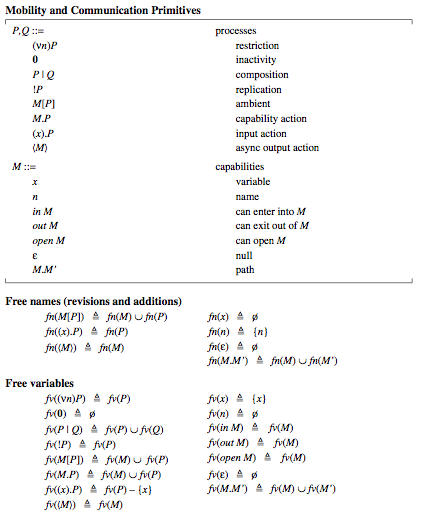
\includegraphics[scale=1]{ambient.png}
  \end{center}
  \captionsetup{justification=centering}  
  \caption{Syntax and scope in the ambient-calculus \\ -- \citep{Cardelli98mobileambients}}
  \label{ambient-syn}
\end{table}

\begin{table} [p]
  \begin{center}
  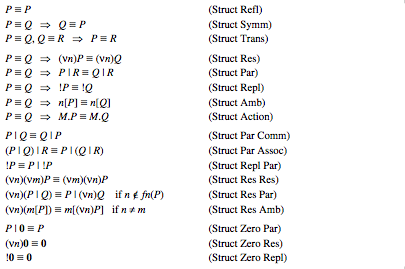
\includegraphics[scale=1]{ambient_str_1.png}
  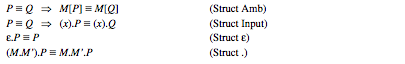
\includegraphics[scale=1]{ambient_str_2.png}
  \end{center}
  \captionsetup{justification=centering}    
  \caption{Structure congurence in the ambient-calculus \\ -- \citep{Cardelli98mobileambients}}
  \label{ambient-str}
\end{table}

\begin{table} [p]
  \begin{center}
  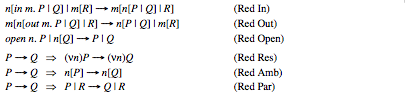
\includegraphics[scale=1]{ambient_red_1.png}
  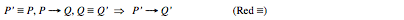
\includegraphics[scale=1]{ambient_red_2.png}
  
\includegraphics[scale=1]{ambient_red_3.png}
  \end{center}
  \captionsetup{justification=centering}    
  \caption{Reduction in the ambient-calculus \\ -- \citep{Cardelli98mobileambients}}
  \label{ambient-red}
\end{table}

\subsubsection{The Obliq Programming Language}
At the time of writing this report, there is no real language that implements the ambient-calculus\footnote{\citet{VMAmbient} proposed a virtual machine for the ambient calculus.}.  Instead,  this section will introduce the Obliq language, which has certain notions of ambient and influenced the design of the ambient calculus.

Obliq\citep{obliq} is one of the earliest programming languages which support distributed programming.  The language was designed before the pervasive of web applications.  It only supports simple object model which is a collection of fields.  Each field of an Obliq object could be a value (a constant or a procedure), a method, or an alias to an object.  An object could either be constructed directly by specifying its fields, or be cloned from other objects.  

The four operations which could be performed on objects are:
\begin{itemize}
  \item selection: a value field of a object could be selected and transmitted over the web.  If the selected value is a constant, the value will be transmitted.  By contrast, if the selected value is a method, values of its arguments will be transmitted to the remote site where the method is defined, the computation is performed remotely, and the result or an exception is returned to the site of the selection.
  \item updating: when an updating operation is performed on an remote object, the selected filed is updated to a value that might be sent across the web.  If the selected filed is a method, a transmission of method closure is required.
  \item cloning: cloning an object will yield a new object which contains all fields of argument objects or raise an error if field names of argument objects conflict.
  \item aliasing:  After executing an aliasing method, a.x := $\bf{alias}$ y $\bf{of}$ b $\bf{end}$, further operations on x of a will be redirected to y of b.
\end{itemize}

It is important to note that Obliq, as some other languages in the pre-web era, does not distinguish local values from distributed values.  By contrast, \citet{dis_note} pointed out that distinct views must be adopted for local and distributed objects, due to differences in latency, memory access, partial failure, and concurrency.
\subsection{The Erlang Language and The OTP Design principles }
\label{sec:Erlang}
%Erlang and OTP Design principles  21 - 25
Erlang \cite{Erlang} is an untyped functional programming language used for constructing concurrent programs.  It is widely used in scalable real-time systems.  The reliability of Erlang systems is largely attributed to the five OTP design principles, namely, supervision trees, behaviours, applications, releases, and release handling \cite{OTP}.  The following subsections will give a brief introduction to the three principles closely related to distributed computing.

\subsubsection{Supervision Trees}
\label{subsec:supervisiontree}

Supervision tree is probably the most important concept in the OTP design principle.  A supervision tree consists of workers and supervisors.  Workers are processes which carry out actual computations while supervisors are processes which inspect a group of workers or sub-supervisors.  Since both workers and supervisors are processes and they are organised in a tree structure, the term $\it{child}$ is used to refer to any supervised process in literature.  An example of the supervision tree is presented in Figure \ref{fig:supervison_tree} \footnote{This example is cited from \href{http://www.erlang.org/doc/design_principles/des_princ.html}{OTP Design Principles/Overview}.  Restart strategies of each supervisor, however, are removed from the figure since they are not related to the central ides discussed here.}, where supervisors are represented by squares and workers are represented by circles.

In principle, a supervisor is accountable for starting, stopping and monitoring its child processes according to a list of $\it{child \ specifications}$.  A child specification contains 6 pieces of information \cite{OTP}: 
\begin{inparaenum} [i)]
  \item a internal name for the supervisor to identify the child. 
  \item the function call to start the child process.
  \item whether the child process should be restarted after the termination of its siblings or itself.
  \item how to terminate the child process.
  \item whether the child process is a worker or a supervisor.
  \item a singleton list which specifies the name of the callback module. 
\end{inparaenum}

\begin{figure}[h]
\begin{center}

\begin{picture}(280, 250)
  \put(15, 70){\circle{30}}
  \put(95, 0){\circle{30}}
  \put(180, 0){\circle{30}}
  \put(260, 0){\circle{30}}
  
  \put(80,55){\line(0,1){30}}
  \put(80,85){\line(1,0){30}}
  \put(110,85){\line(0,-1){30}}
  \put(110,55){\line(-1,0){30}}
  
  \put(200,55){\line(0,1){30}}
  \put(200,85){\line(1,0){30}}
  \put(230,85){\line(0,-1){30}}
  \put(230,55){\line(-1,0){30}}
  
  \put(140,125){\line(0,1){30}}
  \put(140,155){\line(1,0){30}}
  \put(170,155){\line(0,-1){30}}
  \put(170,125){\line(-1,0){30}}
  
  \put(0,125){\line(0,1){30}}
  \put(0,155){\line(1,0){30}}
  \put(30,155){\line(0,-1){30}}
  \put(30,125){\line(-1,0){30}}  

  \put(70,202){\line(0,1){30}}
  \put(70,232){\line(1,0){30}}
  \put(100,232){\line(0,-1){30}}
  \put(100,202){\line(-1,0){30}}  

  \put(180,15){\line(1,1){40}}
  \put(260,15){\line(-1,1){40}}
  \put(95,15){\line(0,1){40}}
  
  \put(95,85){\line(3,2){62}}
  \put(220,85){\line(-3,2){62}}
  \put(15,85){\line(0,1){40}}
  
  \put(15,155){\line(3,2){70}}
  \put(155,155){\line(-3,2){70}}
\end{picture}

\end{center}
\caption{a supervision tree}
\label{fig:supervison_tree}
\end{figure}


\subsubsection{Behaviours}

Behaviours in Erlang, like interface or traits in the objected oriented programming, abstracts common structures and patterns of process implementations.  With the help of behaviours, Erlang code can be divided into a generic part, a behaviour module, and a specific part, a callback module.  Most processes, including the supervisor in \S\ref{subsec:supervisiontree} , could be implemented by realising a set of pre-defined callback functions for one or more behaviours.  Although ad-hoc code and programming structures may be more efficient, using consistent general interfaces make code more maintainable and reliable.  Standard Erlang/OTP behaviours include: 
\begin{inparaenum} [i)]
  \item $\it{gen\_server}$  for constructing the server of a client\-server paradigm. 
  \item $\it{gen\_fsm}$ for constructing finite state machines. 
  \item $\it{gen\_event}$ for implementing event handling functionality. 
  \item $\it{supervisor}$ for implementing a supervisor in a supervision tree. 
\end{inparaenum}
Last but not least, users could define their own behaviours in Erlang.


\subsubsection{Applications}

The OTP platform is made of a group of components called applications.  To define an application, users need to annotate the implementation module with ``-behaviour(application)'' statement and implement the start/2 and the stop/1 functions.  Applications without any processes are called library applications.  In an Erlang runtime system, all operations on applications are managed by the $\it{application\ controller}$ process \footnote{registered as application\_controller}.

This project is concerns in distributed applications which may be used in a distributed system with several Erlang nodes.  An Erlang distributed application will be restarted at another node when its current node goes down.  A distributed application is controlled by both the application controller and the distributed application controller \footnote{registered as dist\_ac}, both of which are part of the $\it{kernel}$ application.  Two configuration parameters must be set before loading and launching a distributed application.  First, possible nodes where the distributed application may run must be explicitly pointed.  Then, all nodes configured in the last step will be sent a copy of the same configuration which include three parameters: the time for other nodes to start, nodes that must be started in given time, and nodes that can be started in given time.

\subsection{Encoding Functions in Process Calculi}
\label{sec:blue}
Process Calculi are used to describe the structure and behaviour of concurrent processes.  As a basis for the design of programming languages, a calculus should be able to encode canonical calculations with functions.  Encoding the $\lambda$-calculus, the canonical form of functional programming, to a processes calculus could be done either indirectly or directly.  

\subsubsection{Indirect Encoding}
In \cite{function_as_process}, Milner gave translation rules from both the lazy $\lambda$-calculus and the call-by-value $\lambda$-calculus to his $\pi$-calculus.  Based on this work, in an higher-order $\pi$-calculus, functions could be encoded into processes and then passed around the network as a value.  Later, Sangiorgi pointed out that the higher-order approach is unnecessary since the plain $\pi$-calculus could simulate this higher-order feature by passing a name that points to the encoding process\cite{HOPI}.

The main drawback of the two indirect encoding approaches is its inefficiency in translation and reduction.  Indirect encoding will yield a mass of intermediate variables.  Moreover, without a direct representation for functions, complex substitutions of variables for functions are unavoidable during reductions.

\subsubsection{The Blue Calculus: Encoding Functions in a Direct Style}
Boudol's blue calculus, $\pi^*$, is a direct extension of both the $\lambda$-calculus and the $\pi$-calculus.  In fact, Boudol defined two calculi in \cite{Blue}: a name-passing $\lambda$-calculus ($\lambda^*$) and an extended $\pi$-calculus without summation and matching ($\pi^*$).  The $\lambda^*$-calculus has $\lambda$-style syntax and $\pi$-style reduction relation (Table \ref{lambda_star}).  It is used as an intermediate language when translating $\lambda$-terms to $\pi^*$-terms.  The $\pi^*$-calculus contains primitives from both the $\lambda^*$-calculus and the $\pi$-calculus so that the translation from both languages is straightforward.

\begin{table} [h]
  \begin{center}
  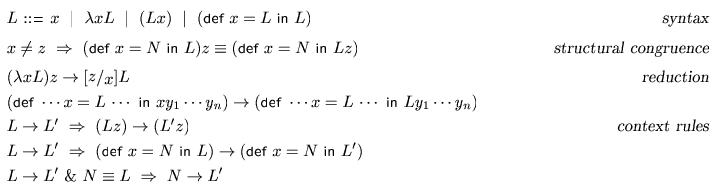
\includegraphics[scale=0.5]{lambda_star.png}
  \end{center}
  \caption{The $\lambda ^*$-calculus}
  \label{lambda_star}
\end{table}

The $\lambda^*$-calculus differs from the $\lambda$-calculus in two aspects:
\begin{inparaenum}[(i)]
  \item The argument ($N$) in an application ($M N$) must be a variable.
  \item A convenient notation for name declaration, $def\ x\ =\ N\ in\ M$, is allowed.
\end{inparaenum}
It is important to note that the $\lambda^*$-calculus only contains the call-by-name evaluation.  This simplifies subsequent studies on relationship between the $\lambda$-calculus and other calculi.  Translations from $\lambda$ to $\lambda^*$ is similar to Launchbury's encoding in \cite{Launchbury93anatural}:

\begin{center}
  \begin{tabular}{ r c l  c}
$x^*$&=&$x$&\\
$(\lambda xM)^*$&=&$\lambda xM^*$&\\
$(M N)^*$&=&$(def\ v = N^*\ in\ (M^*v))$&($v$ fresh)\\
  \end{tabular}
\end{center}

As mentioned earlier, both the $\lambda^*$-calculus and the $\pi$-calculus (without summation and matching) could be translated to the  $\pi^*$-calculus (see Table \ref{trans_blue}).  In addition, a CPS \footnote{continuation passing style} transform from the $\pi^*$-calculus to the $\pi$-calculus is given in \cite{Blue} as well.  Lastly, Silvano Dal-zilio \cite{Dal-Zilio97implicitpolymorphic} proposed a implicit polymorphic type sytem for the $\pi^*$-calculus as an improvement of the original simple type system in \cite{Blue}.

\begin{table}[h]
  \begin{center}
  \begin{tabular}{ l r c l r}
syntax:\\
&$P$&::=& $A\ |\ D\ |\ (P\ |\ P)\ |\ (\nu x)P$&processes\\
&$A$&::=& $u\ |\ (\lambda u)P\ |\ (Pu)$&agents\\
&$D$&::=& $\langle u\ =\ P\rangle\ |\ \langle u\ \Leftarrow P\rangle$& declarations\\
structural equivalence:\\
&$(P\ |\ Q)$&$\equiv$&$(Q\ |\ P)$&commutativity\\
&$((P\ |\ Q)\ |\ R)$&$\equiv$&$(P\ |\ (Q\ |\ R))$&associativity\\
&$((\nu u)P\ |\ Q)$&$\equiv$&$(\nu v)(P\ |\ Q)\ \ (u\ is\ not \ free\ in\ Q)$&scope migration\\
&$(P\ |\ Q)u$&$\equiv$&$(Pu\ |\ Qu)$&distributivity\\
&$((\nu u)P)v$&$\equiv$&$(\nu u)(Pv)\ \ (u\ \neq\ v)$&\\
&$Du$&$\equiv$&$D$&\\
&$\langle u\ =\ P\rangle$&$\equiv$&$\langle u\ \Leftarrow\  (P\ |\ \langle u\ =\ P\rangle )\rangle$&duplication\\
reduction:\\
&$((\nu u)P)v$&$\rightarrow$&$[v/u]P$&$\beta$\\
&$(u\ |\ \langle u\ \Leftarrow\ P \rangle)$&$\rightarrow$&$P$&resource fetching
  \end{tabular}
  \end{center}
  \caption{The $\pi^*$-Calculus}
  \label{blue}
\end{table}

\begin{table}[h]
  \begin{center}
  \begin{tabular}{ r c l r c l}
$[x]u$&=&$\overline{x}u$&$[\overline{u}v_1\cdots v_k]$&=&$uv_1\cdots v_k$\\
$[\lambda xL]u$&=&$u(x,v)[L]v$&$[u(v_1, \cdots ,v_k)P]$&=&$\langle u\ \Leftarrow\ (\lambda v_1 \cdots v_k)[P]\rangle$\\
$[Lx]u$&=&$(\nu x)([L]v\ | \ \overline{v}xu)$&$[!u(v_1, \cdots ,v_k)P]$&=&$\langle u\ =\ (\lambda v_1 \cdots v_k)[P]\rangle$\\
$[def\ x\ =\ N\ in\ L]u$&=&$(vx)([L]u\ |\ !x(v)[N]v)$&$[P\ |\ Q]$&=&$([P]\ |\ [Q])$\\
&&&$[(\nu u)P]$&=&$(\nu u)[P]$
  \end{tabular}
  \end{center}
  \caption{Translation from $\lambda^*$-calculus and $\pi$-calculus to $\pi^*$-calculus}
  \label{trans_blue}
\end{table}

\subsection{Implementation Strategies}
\label{sec:vanroy}

This section will give a short survey on Peter Van Roy's general framework for the implementation of concurrent programming languages  \cite{Roy06convergencein, roy}.  \cite{Roy06convergencein} abstracts a four-layer-structure which smoothly applies to four languages designed for different purposes.  The four-layer-structure and case studies in \cite{Roy06convergencein} are summarized in Table \ref{layer}.  The rest of this section will introduce the main results in \cite{roy}, which is focused on implementation details.

\begin{table}
  \begin{center}
  \begin{tabular}{| l | c | c | c | c |}
\hline
Layer&      Erlang   &    E   &    Mozart  &Oz\\
\hline
strict functional language          &Y&Y&Y&Y\\
\hline
deterministic concurrency          & N&Y&unknown&Y\\
\hline
asynchronous message passing&Y&Y&Y&Y\\
\hline 
global mutable state                     &Y&N&Y&Y\\  
\hline
  \end{tabular}
  \end{center}
  \caption{a shared structure for 4 programming languages}
  \label{layer}
\end{table}


\subsubsection{A General Purpose Virtual Machine}
The basic abstract machine in \cite{roy} consists of three elements: statement $\langle$s$\rangle$, environment E, and assignment store $\sigma$.  Explanations for concepts related to this VM are given as follows:
\newpage
\begin{itemize}
  \item an {\it{assignment store  $\sigma$}} contains a set of variables.  Variables could be bound, unbound, or partially bound.
  \item an {\it{environment}} E stores mappings from variable identifiers to entities in $\sigma$.
  \item a {\it{semantic statement}} is a pair of ($\langle s \rangle$, E).
  \item an {\it{execution state}} is a pair of (ST, $\sigma$), where ST is a stack of semantic statements.
  \item a {\it{computation}} is a sequence of transitions between execution states.
\end{itemize}

\subsubsection{Extending the Basic VM}
\label{ex_vm}
The basic VM described in the last section is capable to model most of computation paradigms directly or indirectly.  More pleasantly, several restrictions and extensions could be added to this basic VM on demand.
\begin{itemize}
  \item MST(multiset of semantic stacks).  Concurrent programming would be supported via simply replacing the ST by MST.  Using the multiset structure for storing semantic stacks gives the flexibility of coordinating identical threads.
  \item bound or unbound variables.   In the book, unbound variables refer to variables which have not been assigned a value.  In sequential computing, unbound variables should not be allowed since the program will be halting forever.  In concurrent computing, however, unbound variables are acceptable since it might be bound by another thread later.
  \item single-assignment variable or multiple-assignment variable.  Although using single-assignment variable should be encouraged to avoid side-effects, multiple-assignment variable may ease the implementation of imperative languages.  Alternatively, both kinds of variable could appear in the same language, such as the Scala language, with different notations.
  \item variable’s lifetime.  There are three moments in a variable’s lifetime. i) creation, ii) specification, and iii) evaluation.  Adjacent moments may or may not be happen at the same time.  Different combinations yields Table \ref{var_life} cited from \cite{roy}.
  \item more kinds of stores.  If the state of a shared store could be regarded as the status of a program, evaluation rules on store variables implies features of the programming paradigm.  The first three examples in the next subsection demonstrate this idea.
  \item new statement syntax.  When the encoding  of certain feature is expensive within the current kernel syntax, adding a new form of statement is one of the easiest way to increase the expressiveness of the language.  The gained expressiveness, however, may not be free.  For example, the number evaluation rules will be increased dramatically and reasoning about programs will be more complex.  Moreover, properties enjoyed by the old model may no longer be hold in the new one.
\end{itemize}

\begin{table} [h]
  \begin{center} 
  \begin{tabular}  {|m{2.5cm} |m{3 cm} |m{3 cm} | m{3 cm} |}
    \hline
    &sequential with values&sequential with values and dataflow variables&concurrent with values and dataflow variables\\
    \hline
   eager execution&strict functional programming&declarative model&data-driven concurrent model\\
  &(e.g., Scheme, ML)&(e.g., Prolog)&\\
  & (1)\&(2)\&(3)&(1),(2)\&(3)&(1),(2)\&(3)\\
    \hline
  lazy execution & lazy functional programming & lazy FP with dataflow variables & demand-driven concurrent model\\
  & (e.g., Haskell) &&\\
  & (1)\&(2),(3) & (1),(2),(3)&(1),(2),(3)\\ 
  \hline
  \multicolumn{4}{l}{}\\
  \multicolumn{4}{l}{(1): Declare a variable in the store}\\
  \multicolumn{4}{l}{(2): Specify the function to calculate the variable's value}\\
  \multicolumn{4}{l}{(3): Evaluate the function and bind the variable}\\
  \multicolumn{4}{l}{}\\
  \multicolumn{4}{l}{(1)\&(2)\&(3): Declaring, specifying, and evaluating all coincide}\\
  \multicolumn{4}{l}{(1)\&(2),(3): Declaring and specifying coincide; evaluating is done later}\\
  \multicolumn{4}{l}{(1),(2)\&(3): Declaring is done first; specifying and evaluating are done later and coincide}\\
  \multicolumn{4}{l}{(1),(2),(3): Declaring, specifying, and evaluating are done separately}\\
  \end{tabular}
  \end{center}
  \caption{Popular computation models in languages}
  \label{var_life}
\end{table}

\subsubsection{Example Paradigms}
Following are 5 examples chose from \cite{roy}.  Each example demonstrates how a popular modern programming feature could be implemented with techniques described in \S \ref{ex_vm}.
\begin{itemize}
  \item Laziness could be realised by adding a need-predict store.
  \item Message passing concurrency could be realised by adding a mutable store, together with two primitives NewPort and Send.
  \item Explicit state could be realised by introducing a mutable cell store.  A cell records a mapping from a name value to a store variable.  Although a name value might be mapped to different store variables at different time, changes to name-variable mapping will not affect the internal state of a program.
  \item Relational programming could be realised by adding choice and failure statements to kernel.
  \item  Constraint programming could be realised by adding a constraint store and a batch of primitive operations.
\end{itemize}


The book  \cite{roy} provides at least two prominent contributions.  Firstly, it provides a framework which unifies most of popular programming paradigms.  Secondly, combining different versions of statements, environment and assignment store yields different programming models.  To the author of this research proposal,  those three components  are three dimensions of the ``language space''.  Researchers in the area of programming languages could use this coordinate system is two ways.  On the one hand, it provides a convenient formalism to compare different programming languages.  On the other hand, regardless of their usages,  new programming paradigms could be defined by filling ``blank coordinates'' of the space.  In fact, some models in the book does not correspond to any well known languages.
